\documentclass[12pt,a4paper]{article}
\usepackage[abbreviate = true, doi = true, style = nature, giveninits = true, sorting = none, backend = biber]{biblatex}
\usepackage[lmargin = 4cm, rmargin = 4cm, tmargin = 2.5cm, bmargin = 2.5cm]{geometry}
\usepackage[onehalfspacing]{setspace}
\usepackage{graphicx}
\usepackage{hyperref}
\usepackage{times}
\usepackage[UKenglish]{babel}
\usepackage[textsize=tiny]{todonotes}
\usepackage[acronym]{glossaries}

\AtBeginBibliography{\small}
\addbibresource{main_sources.bib}

\setlength{\parindent}{0cm}
\setlength{\marginparwidth}{3.5cm} % make todonotes wider
\newcommand{\todoleft}[1]{{\reversemarginpar \todo{#1}}}
% preset for italic species name, abbreviated after first use
\newacronym[first = {\textit{Harmonia axyridis}}]{harm}{\textit{H. axyridis}}{\textit{Harmonia axyridis}}
\glsdisablehyper % no hyperref for \gls

%%%%%%%%%%%%%%%%%%%%%%%%%%%%%%%%%%%%%%%%%%%%%%%%%%%%%%%%%%%%%%%%%%
\begin{document}

\title{Thesis}
\author{Lukas Prader}
\date{\today}
\maketitle

\newpage
\tableofcontents
\newpage

\section{Introduction}
 (citations missing)

The topic of invasive species has become more and more important, even more so with recent changes in climate and habitats due to human influence.
In order to deal with invasive species and the impact they can have on existing ecosystems, species distribution models (SDMs) have been used to predict the potential habitat and with that the threat of an emerging invasive species.
Especially time-partitioned models can provide more insight into the process of invasion.
Ensemble models are often used in applications where models are projected, since aspects of different modelling approaches can be combined to hopefully gain a more complete model of the species distribution.

There are certain challenges when using SDMs in invasive research though.
For example, the invading species is usually not currently in equilibrium with its environment, leading to underestimations of the final niche occupied.
A similar difficulty is modelling the invaded range with data from a species native range since the native niche can be quite different from the realized invaded niche.
Nonetheless, SDMs are frequently used in trying to predict the spread of invasive species, which is why it is important to gain a better understanding of invasion processes and an SDM's ability to accurately represent it.

\gls{harm}, also known as the harlequin or Asian lady beetle, is an invasive species already established in non-native habitats all around the world.
The invasion process has already been studied extensively and there have been SDMs modelling the invaded range in Europe as well, though mostly on a national scale.

One goal of this thesis is to look into the limitations of models built early in the invasion process of a species.
By iterating over the years of the invasion, model performance can be evaluated with consideration to the current state of invasion.
Computing the occupied niche separately for each year also provides more insight into the invasion process and might help to understand modelling limitations for certain years.

\newpage
\section{Methods}
 (citations missing)
\subsection{Datasets}
For occurrence data, all global occurrences of \gls{harm} were downloaded from the GBIF database \autocite{GBIFaxyridisdataset}.
All traditional 19 bioclim variables were obtained from the CHELSA V2.1 climatologies dataset \autocite{karger2017CHELSApaper, CHELSAbioclimdataset}, using the 1981-2010 time frame for all years from 2002 to 2010 as well as the MPI-ESM 1.2 ssp370 scenario 2011-2040 for all years from 2011 to 2022.
In order to also have some kind of influence of the human nature of first introduction, land cover data was used from the Copernicus Land cover Classification dataset \autocite{COPlandcoverdataset}  with yearly resolution for 2002 up to 2020.

\subsection{Data preparation}
All bioclim and land cover layers were resampled to a matching resolution of 30 arc seconds and cropped to two spatial extents, Europe and the presumed native range referencing (Orlova-Bienkowskaja, Ukrainsky \& Brown, 2015) \autocite{orlova2015harmonia}.

The presence-only points from GBIF were checked for missing values for latitude, longitude, year or coordinate uncertainty and then subset to the afore mentioned spatial extents.
No occurrences after 2022 were used, also no points with a coordinate uncertainty larger than 1 km.
In Europe, the initial cut off year for presences was 1991, since this is the year of invasion according to the EASIN website.
Afterwards, using the library \texttt{CoordinateCleaner}, all remaining data points were again checked for common errors or biases in the respective subset (tests used: "capitals", "centroids", "duplicates", "equal", "institutions", "outliers", "seas", "zeros").
In addition, all occurrences were checked for their land cover class values in their respective year, removing points in the water or with no data.
In the end, remaining data points prior to 2002 were deemed insignificant and removed from the dataset.
To prepare the data for modelling, pseudoabsences were generated for each year, randomly sampling the area and resampling points in the water or with no data.

\subsection{Model building}
For each year, the following Models were computed: General Linear (GLM), General Additive (GAM), Boosted Regression Trees (BRT) and Maximum Entropy (MAXENT).
A model for a specific year always included all points from past years as well.
The iterative models that were built only use data points from Europe, though there was one model created only with native occurrences and predicted for each year in Europe.
For all used occurrence points after 2020, the land cover data of 2020 was used as a substitute.

Variance inflation factors were used to select the variables used for model building.
For this, a GLM was computed only using Europe data from 2022.
This model included all 19 bioclim variables and their squared values as separate variables.
For land cover variables, a PCA was computed on the relative area of all land cover classes in an 18 km radius around an occurrence point.
The 18 km radius was chosen, since it is the average flight distance determined for \gls{harm} \autocite{jeffries2013flightharmonia}.
PCA axes were included in the model until a cut-off of 80\% of explained variance was reached.
Variance inflation factors were computed for this GLM and the variable with the highest VIF was dropped until none of the remaining variables had a VIF greater than 10. 
Quadratic versions of bioclim variables were always dropped before their linear counterparts, even if their VIF was lower.

\subsection{Analysis}
All SDM models of each year were evaluated for their accuracy on predicting the occurrences of the following year and the final year of 2022 using the True Skill Statistic (TSS).
The TSS values were used to create a TSS-weighted ensemble of all model predictions, which was again evaluated for its accuracy.
For each year, the occupied niche was computed by running a PCA analysis on the bioclim variables.
The niche can then be visualized by plotting a dynamic occurrence density grid for the first two PCA axes \autocite{broennimann2012niche}.
The overlap between each year for Europe and the respective following year was computed, as well as a niche similarity and niche equivalency test.
Niche overlap for each year was also visualized in comparison to the total native niche.
All mentioned niche analyses were conducted using the library \texttt{ecospat} \autocite{dicola2017ecospat}.



\newpage
\section{Background}
This section aims to give sufficient background on \gls{harm} and the theory necessary to understand this thesis.

\subsection{Invasion theory}
The Invasive Alien Species Regulation of the European Union from 2014 uses the following definitions for alien species and invasive alien species \autocite{EU2014LexIAS}:
\begin{quote}
    (1) 'alien species' means any live specimen of a species, subspecies or lower taxon of animals, plants, fungi or micro-organisms introduced outside its natural range; it includes any part, gametes, seeds, eggs or propagules of such species, as well as any hybrids, varieties or breeds that might survive and subsequently reproduce;

    (2) 'invasive alien species' means an alien species whose introduction or spread has been found to threaten or adversely impact upon biodiversity and related ecosystem services;
\end{quote}

This already shows the main concerns associated with invasive species, non-native species that have an often negative impact on native ecosystems.
Main goals in research are to find out which species have potential to become invasive, what habitat will be susceptible to invasion by those species, how fast the species will invade the new area and what impact its invasion will have on the native ecosystem \autocite{shigesada1997invasions}.
To this end, many theories have been created to describe invasion processes.
The invasion of a species can  generally be described with four stages \autocite{blackburn2011invasionstages}:
\begin{enumerate}
    \item Transport: Leaving the native range, arriving at a new location
    \item Introduction: Existing in specific locations (captivity / cultivation)
    \item Establishment: Existing outside of areas of introduction in the wild
    \item Spread: Sustaining establishment and dispersing to new environments
\end{enumerate}

The impacts of invasive alien species can be numerous, ranging from food web changes to reductions in habitat and species richness, hydrology and nutrient cycle changes, enhanced invasion of other species and mass extinctions \autocite{simberloff2013invasiveimpacts}.
For example intraguild predation, the predation of species using similar resources, can create completely new stable states of an ecological system \autocite{polis1989theoryIGP}.

\subsection{Species Distribution Modelling}
Species Distribution Models (SDMs) attempt to connect species distribution data, i.e. occurrence at a location, to the environmental and spatial properties of said location \autocite{elith2009sdmtheory}.
They have been shown to generate substantial insight into the ecological requirements of species and, as niche models, can be used to predict the potential habitat of a species \autocite{araujo2006sdmchallenges}.
There has been considerable debate on the capabilities and limitations of SDMs, especially when used for prediction.
In general, SDMs are made with the (ideal) assumption that the species is in environmental equilibrium \autocite{elith2009sdmtheory}, implying that its ecological niche is not currently changing.
If these models are now used to predict new, unsampled areas, there actually is no measure to assess their accuracy, since no data is presently available for that area \autocite{araujo2006sdmchallenges}.
There is also no guarantee that the biotic interactions sampled in the study area will reflect the final interactions in the new area \autocite{elith2009sdmtheory}.
All of these issues apply especially to the prediction of invasive species, since there might be limited data in the invaded range, the species is often not currently at equilibrium and interactions with native species are completely new \autocite{mainali2015sdmprojecting}.
Despite all these challenges, SDMs have been used numerous times to provide insight into the invasive potential and the invasion dynamics of alien species \autocite{zimmermann2010sdmtrends}.
One way of gaining more insight into the invasion process is to create models with data from different time periods during the invasion \autocite{briscoe2019palmerisdm}.
For example, data from a time period early in the invasion process can be used to build models which then are evaluated against data from a later time period \autocite{barbet2018nigrithoraxsdm}.

\subsection{Modelling methods}
A diverse array of mathematical models have been developed to describe ecological processes.
In species distribution modelling, several modelling methods have emerged with differing strengths and weaknesses, including the following:

\textbf{Generalized Linear Models (GLM)} \autocite{nelder1972glm}:\\
GLMs are the generalized extension of a classical linear model, meaning a linear combination of all used variables in the form of
\begin{equation}
    \label{eq:lm}
    Y = \beta_1 x_1 + \beta_2 x_2 + \dots = \sum_{i} \beta_i x_i,
\end{equation}
where $Y$ is the final response value, $x_i$ are the independent variables used in the model and $\beta_i$ are the parameters that need to be estimated for each variable.
This can now be generalized for non-linear relationships between the variables and the response value, for example the expectation values of a statistical distribution.
A link function $g$ (non-linear), is applied to the response in order to match the results of the (still linear) combination of model variables to a desired statistical distribution (i.e. normal, binomial, Poisson, gamma), resulting in
\begin{equation}
    \label{eq:glm}
    E = g(Y) = \sum_{i} \beta_i x_i .
\end{equation}
With this transformation, $g(Y)$ now represents the expectation value $E$ for the model in the chosen distribution.

\textbf{Generalized Additive Models (GAM)} \autocite{hastie1986gam}:\\
A GAM can be understood as an even further extension of a GLM. Here, variables are not estimated with a linear parameter any more, but are each contained in a "smooth function" $s()$:
\begin{equation}
    \label{eq:gam}
    E = \sum_{i} s_i(x_i)
\end{equation}
The smooth functions are estimated non-parametrically, meaning that the form of $s()$ is not strictly predefined in comparison to GLMs, where $\beta_i$ is clearly a simple parameter to be estimated.
The smooth function could for example be estimated using splines, piecewise defined polynomial functions.
Both GLMs and GAMS are fundamental advancements in statistical regression and have been used heavily in ecological research \autocite{guisan2002glm-gam}.

\textbf{Boosted Regression Trees (BRT)} \autocite{elith2008brt}:\\
BRTs are a form of machine learning model using multiple decision trees and boosting to create a well performing model.
Tree based models can be used for classification or regression tasks.
Decision trees fit a constant value to intervals of all variables, either the most probable class (classification) or the mean response (regression) of all observed values in that interval.
\begin{figure}[!h]
    \centering
    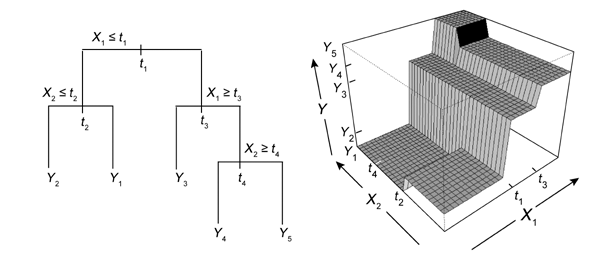
\includegraphics[width = 0.95\linewidth]{figures/elith-brt.png}
    \caption{\label{fig:elith_brt} Visualization of a decision tree (left) and the resulting response surface for the two variables $X_1$ and $X_2$. (modified from \autocite{elith2008brt})}
\end{figure}

Multiple decision trees can be combined using boosting to generate a tree ensemble with much better performance.
Here, a first tree is built trying to maximize the prediction accuracy for the fitted values.
All following trees are generated with emphasis on values that are not well described by the current amount of trees.
This can be done by applying weights to those values for the next tree.
When using BRTs for regression, boosting can be understood as optimizing the residuals of the fit function, the difference between the observed value and the estimated value.
Each tree usually only contributes a very small amount to the total result, scaled by a so-called learning rate.
BRTs have the potential to strongly overfit the data, meaning that the resulting function is very accurate for the used training data, but much less so for new data not used in the training process.

\textbf{Maximum Entropy Method (MaxEnt)} \autocite{phillips2006maxent, phillips2017maxnet}:\\
Maximum Entropy at its core is an optimization method commonly used in machine learning.
It follows the concept that as few constrains as possible should be used when modelling a distribution that is currently unknown.
This is achieved by maximizing the "entropy" of the estimation, here meaning a measurement for the amount of constraints influencing the result.
In MaxEnt SDMs, variables are added in form of "features" representing different constraints put on the model for a specific variable:
\begin{itemize}
    \item Linear feature: The mean of the response should be close to the observed value.
    \item Quadratic feature: The variance of the response should be close to the observed value.
    \item Product feature: The covariance of two variable responses should be close to the observed value.
    \item Threshold feature: The proportion of response values above a given threshold should be close to the observed value.
    \item Binary feature: The proportion of response values belonging to a certain binary value should be close to the observed value (for categorical data).
    \item Hinge feature: A piecewise linear function imposing constraints similar to the threshold feature.
\end{itemize}

MaxEnt models also use regularization, a process that puts penalties on complex models and produces a simpler model (fewer and less complex coefficients).
It has recently been shown that MaxEnt models can be fit using infinitely weighted logistic regression, making it very similar to GLMs and GAMs in its concept, apart from the use of "features".
\\
Due to differing strengths and weaknesses of each modelling method, a possible approach is to create an ensemble of multiple models \autocite{araujo2007ensemble}.
The way of combining model predictions can vary, but the goal is to improve total performance by combining the results of all computed models.

\subsection{Harmonia axyridis}
\gls{harm}, also known as the Harlequin ladybird or multicoloured Asian lady beetle, is of the family of the Coccinellidae and has its native origin in Asia \autocite{roy2016harmonia}.
At first widely introduced as a control species against pest aphids, \gls{harm} has turned out to be a highly invasive species reaching an almost global distribution \autocite{brown2008harmonia}.
In America, the species was introduced as early as 1916 (California) and in 1988, first populations outside intended release were found \autocite{chapin1991harmoniaNA}.
Usage of \gls{harm} for biological control in Europe dates back as far as 1990 (France) \autocite{coutanceau2006harmoniaFR}.
First invasive occurrences were confirmed in multiple countries during the early 2000s, including Germany (2000), Belgium (2001), the Netherlands (2002) and the United Kingdom (2003) \autocite{roy2016harmonia}.
The first confirmation in Austria, where it was never used for biological control, was 2006 \autocite{rabitsch2006harmoniaAT}.
It has been shown that all established invasive populations outside of North America have their origin in the first established population in eastern North America, with the European populations being significantly influenced by the used biocontrol strain \autocite{lombaert2010harmoniabridgehead}.

The impact of \gls{harm} on invaded areas is diverse.
In some contexts, the ladybird has been shown to have a negative impact on the diversity and abundance of native ladybird species \autocite{roy2016harmonia}.
Many studies show intra guild predation and direct interspecific competition in favour of \gls{harm} \autocite{pell2008harmoniaIGP}.
It has also been shown that the species feeds on a variety of damaged fruit crops, for example grapes, apples, stone fruit and berry crops \autocite{koch2004harmoniafoodcrop}.
The aggregating behaviour of \gls{harm}, mostly as a strategy for overwintering, is also a cause of disturbance, since private homes and facilities are invaded by large amounts of beetles at a given time \autocite{nalepa2005harmoniahomes}.

\newpage
\printbibliography[]
\newpage
\appendix
Appendix

\end{document}